\documentclass[11pt]{article}
\usepackage[left=1in,right=1in,top=0.75in,bottom=0.75in]{geometry}
\usepackage{amsmath}
\usepackage{graphicx}
\usepackage{float}
\usepackage[hidelinks]{hyperref}
\usepackage{microtype}

\begin{document}

Hello professor, here is a higher level overview of the projects I have been working on since being admitted to your group this recent January. This report also indicates how Jacopo and I have visualized the subsequent work-load/paper trajectories, and the preliminary results of each so far.

As a brief note on workload, last semester I took two courses in addition to your research credit, while being enrolled as a teacher assistant for Physics 104 with the responsibility of discussions 4x/week and labs 2x/week along with substituting for other TAs. I am enrolled in a course this summer.
or workload, there were numerous nights that I slept at the Physics office to save commute time (although now I live only 4 blocks away from the MSE building).

Here is what I have worked on and the road-map:

\subsubsection*{Paper I: ADAPT-VQE Ground State}
My algorithm ranks operators ($A$) by energy per cost $\Delta E / K$ within a position $p$ of the current ansatz circuit $U(\theta)$. So I write the pair as:
\[
r=(A,p) \mapsto e^{i\alpha A} \mapsto U(\theta)| \phi_{\rm ref} \rangle=|\psi\rangle.
\]
Novelty:

- Shortlisting of records to get higher order energy modeling with number of quantum measurements less than scoring/modeling the full operator pool.

- Scoring operators per unit hardware cost.

- Insertion was recently introduced by GEO-ADAPT this May, but they found little benefit in their algorithm, whereas mine establishes more benefit and also the activation of insertion-scoring occurs during energy-gradient plateaus which likewise saves costs.

- Operator pool definition for Hubbard--Holstein model with high physical response channel relevance.

- Energy model for adding multiple operators at once, energy model for deleting an operator from $U(\theta)$, and the first application of Lowrerre beam search to ADAPT-VQE.

- Gram matrix which allows for Trust-region based modeling, and allows for the whitening of coordinates (produces orthonormal basis on retained non-null tangent support) which helps inner optimization procedures.


\subsubsection*{Paper II: Time Dynamics of Hubbard--Holstein}
This project time-evolves a Paper-I ground-state ansatz with the McLachlan variational principle. The main additions are:

- State-space numerical stabilization through regularized linear solves and local time-step subdivision.

- Cost-weighted addition and deletion of ansatz generators during propagation. Adaptive addition already exists in the literature; to the best of my current search, online generator deletion during McLachlan dynamics does not.

- Quantum simulation of driven Hubbard--Holstein energy, site occupations, and doublon dynamics.

Figure~\ref{fig:paper-ii-results} uses the same redundant 118-parameter ansatz, Gaussian drive ($A=0.8$), and time grid through $t=5$ for all three comparisons. Reductions relative to fixed McLachlan are:

\begin{center}
\small
\begin{tabular}{lrrrr}
\hline
Method & \shortstack{Energy-error\\reduction} & \shortstack{Doublon-error\\reduction} & \shortstack{Parameter\\reduction} & \shortstack{$N_{2q}$\\reduction} \\
\hline
Stabilization & $14.5\%$ & $47.9\%$ & $0\%$ & $0\%$ \\
Stabilization + pruning & $37.0\%$ & $70.3\%$ & $24.6\%$ & $33.0\%$ \\
\hline
\end{tabular}
\end{center}

\begin{figure}[H]
    \centering
    \small\textbf{Legend:} blue: McLachlan propagation; orange and green: exact references; pale bands: numerical stabilization; red diamonds: accepted deletions.
    \par\medskip
    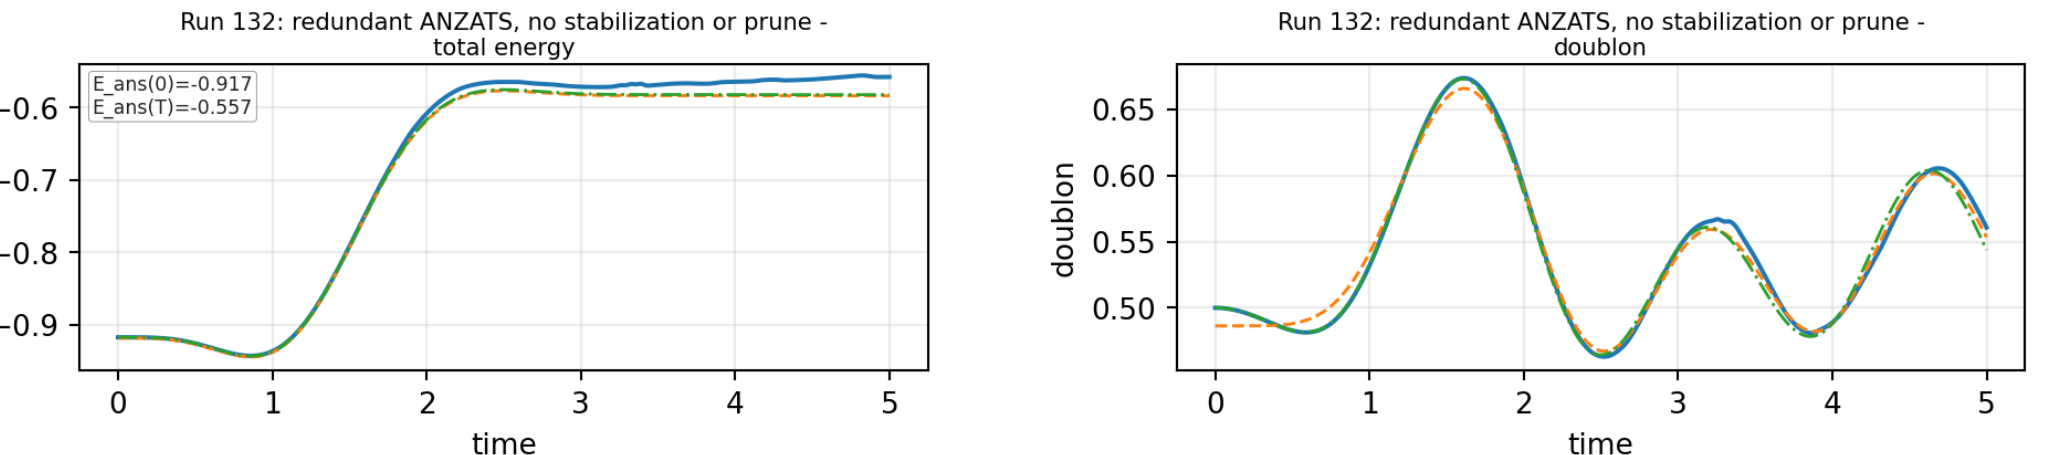
\includegraphics[width=0.80\linewidth]{advisor_project_overview_assets/results_pdf_crops/run132_fixed_energy_doublon.png}
    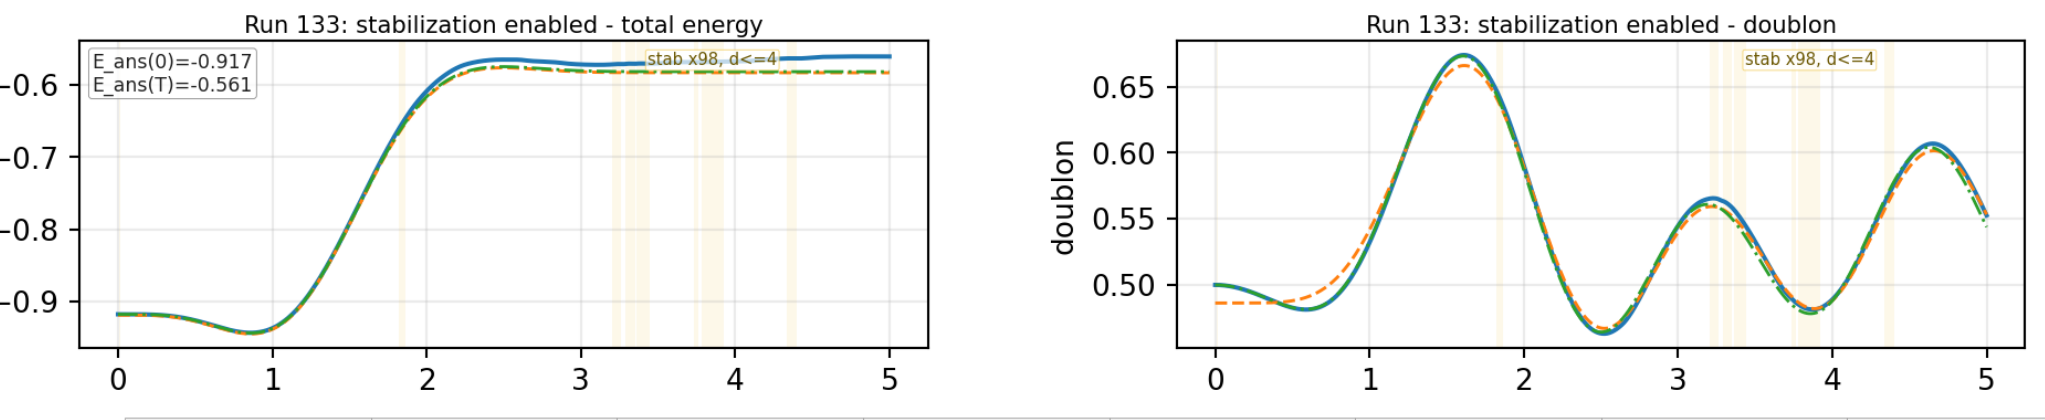
\includegraphics[width=0.80\linewidth]{advisor_project_overview_assets/results_pdf_crops/run133_stabilization_energy_doublon.png}
    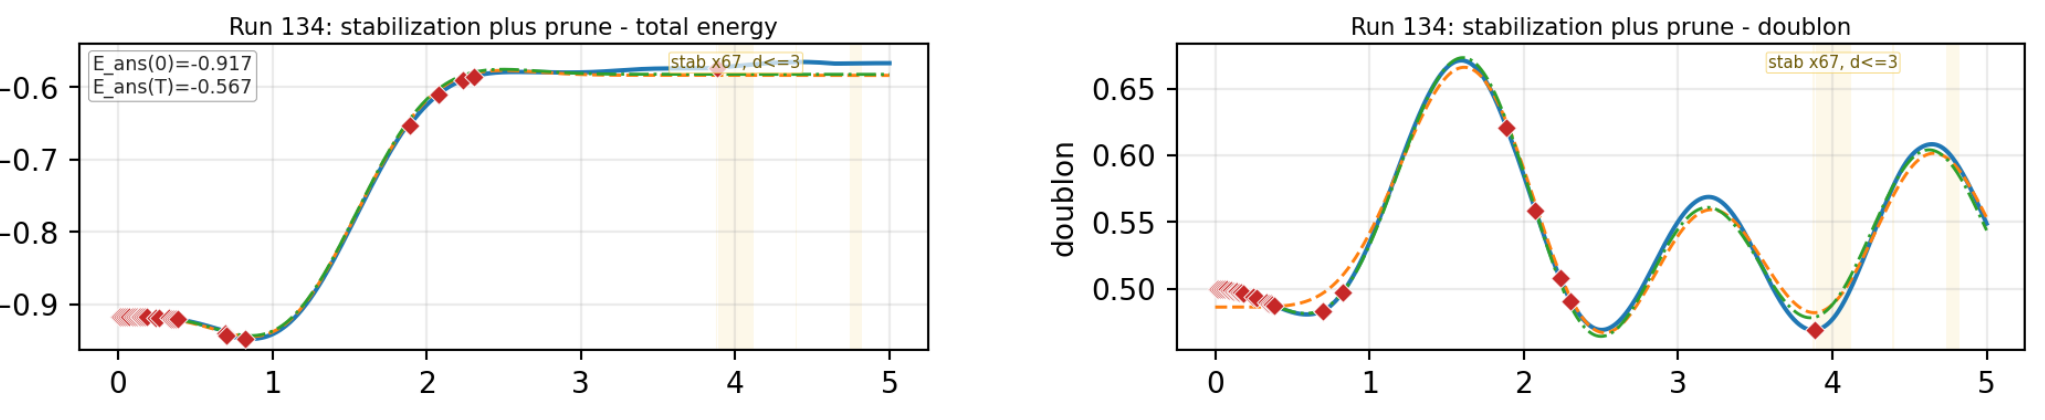
\includegraphics[width=0.80\linewidth]{advisor_project_overview_assets/results_pdf_crops/run134_stabilization_prune_energy_doublon.png}
    \caption{Total energy and doublon trajectories from the Results PDF: fixed McLachlan (top), numerical stabilization (middle), and numerical stabilization with pruning (bottom).}
    \label{fig:paper-ii-results}
\end{figure}

\subsubsection*{Paper III: Quantum Subspace Expansion and Excited-State Dynamics}
From a source-locked RA-ADAPT ground state, response-operator QSE for the half-filled two-site Hubbard--Holstein model with \(n_{\rm ph}^{\max}=3\) reproduces the exact first-excitation gap (\(0.865200327\) versus \(0.865200264\)) with state fidelity \(0.999999983\). Figure~\ref{fig:paper-iii-promoted-ap} compares driven AP-McLachlan with fixed McLachlan, which holds the same initial 30-generator support unchanged while AP-McLachlan enlarges it during propagation. Current work targets collective support selection and compact geometry- and cost-selected QSE.

\begin{figure}[H]
    \centering
    
\includegraphics[width=0.82\linewidth]{advisor_project_overview_assets/paper_iii/paper_iii_promoted_ap_diagnostic.pdf}
    \caption{Driven response of the first QSE excited state under the same drive, \(A=0.05\) and \(\omega=0.865200327\): exact Schr\"odinger propagation (black), AP-McLachlan (orange), and fixed McLachlan (gray dashed). ``AP'' denotes adaptive generator support; both McLachlan trajectories use the fixed fourth-order Runge--Kutta step \(\Delta t=0.025\,T_{\mathrm{hop}}^{-1}\). They start with the same 30 generators; fixed McLachlan holds them unchanged, whereas AP-McLachlan admits additional generators. The exact reference is propagated independently in the fixed-particle sector under the driven Hamiltonian and sampled at the same plotted times. Panels show the staggered density (a), staggered phonon displacement (b), and fidelity to the exact state (c) through \(t=10\,T_{\mathrm{hop}}^{-1}\). AP-McLachlan grows from 30 to 330 parameters through 106 accepted support updates and raises the minimum exact-state fidelity from \(0.9209\) to \(0.9879\). Its maximum density and displacement errors are \(0.0352\) and \(0.0978\), compared with \(0.1033\) and \(0.1456\) for fixed McLachlan.}
    \label{fig:paper-iii-promoted-ap}
\end{figure}

\subsubsection*{Paper IV}
Applying the paper I and II (and likely iii) algorithms to a real molecular system, such as the vibronic H2O molecule, which I have computed using Psi4 and matched Doron's results under equal geometry. I have synced it to my Paper I algorithmic-route already and have been running it for a few hours now. This direction was adviced from Jacopo and so I am less clear on the novelty aside from the fact that it is a new hamiltonian problem, and will use the unique algorithm routes Paper I through III developed.

\clearpage
\subsubsection*{Paper V: Representability-Preserving Electron--Phonon Dynamics}
This project investigates a quantum-algorithmic treatment of the equal-time electron--phonon equations in \href{https://arxiv.org/abs/2606.22233}{``Open-quantum-system theory of non-Markovian electron--phonon dynamics.''} As a classical prerequisite, I reproduced the reported strong-coupling instability using the 13 real variables obtained by imposing the dimer symmetries on the source equations. A coordinate exceeded \(10^4\) at \(t=130.47\,t_{\mathrm{hop}}^{-1}\), whereas the tested weak-coupling trajectory remained bounded through \(t=140\,t_{\mathrm{hop}}^{-1}\). Retaining the complete matrix structure and imposing unit trace, Hermiticity, and covariance symmetry leaves 31 independent real variables. At 100 random states and times, their derivatives agreed with an independent evaluation of the source matrix equations to floating-point precision.

The retained objects are the electronic density \(\rho_{ij}=\langle c_j^\dagger c_i\rangle\), coherent phonon amplitudes \(B_q=\langle b_q\rangle\), normal and anomalous phonon moments \(N_{qr}=\langle\delta b_r^\dagger\delta b_q\rangle\) and \(A_{qr}=\langle\delta b_q\delta b_r\rangle\), and connected electron--phonon correlations \(C^q_{ij}=\langle\delta b_q(c_j^\dagger c_i-\rho_{ij})\rangle\), where \(\delta b_q=b_q-B_q\). Their joint Gram matrix has the block structure
\[
\mathcal G(\rho,N,A,C)=
\begin{pmatrix}
M_{\mathrm B}(N,A)&Z(C)\\
Z(C)^\dagger&E(\rho)
\end{pmatrix}\succeq0,
\qquad
M_{\mathrm B}(N,A)=
\begin{pmatrix}
N^{\mathsf T}&A^*\\
A&I_2+N
\end{pmatrix},
\]
Here \(Z(C)\) is the \(4\times3\) cross-Gram block between the centered phonon directions \((\delta b_0,\delta b_1,\delta b_0^\dagger,\delta b_1^\dagger)\) and centered electronic Pauli directions \((\delta\sigma_x,\delta\sigma_y,\delta\sigma_z)\), while \(E(\rho)\) is the \(3\times3\) Gram matrix of the latter, with \(\delta\sigma_a=\sigma_a-\operatorname{Tr}(\rho\sigma_a)I_2\), for \(a\in\{x,y,z\}\). Physical representability requires positive semidefiniteness of \(\mathcal G\) together with the fixed-particle-number conditions \(\operatorname{Tr}C^q=0\). In one consistent 31-variable protocol, the uncorrected equations violated positive semidefiniteness of \(\mathcal G\) at \(t=0.1607\,t_{\mathrm{hop}}^{-1}\) and of \(M_{\mathrm B}\) at \(t=3.6821\,t_{\mathrm{hop}}^{-1}\), long before the late amplitude divergence. At every Runge--Kutta evaluation, I added the minimum-Euclidean-norm correction \(w\) to the 31-component velocity, subject to the electronic and joint-Gram positivity constraints, the correlation-trace conditions, and zero correction-induced energy flux. The resulting constrained quadratic program propagated successfully through \(t=1000\,t_{\mathrm{hop}}^{-1}\), with all 400,000 constrained evaluations converged, positive margins above \(2.06\times10^{-5}\), and maximum post-pulse energy change \(5.03\times10^{-6}\). To test closure accuracy separately, I compared \(\dot C_{31}\), the \(C\)-block of the uncorrected 31-variable velocity, with \(\dot C_{\mathrm{ex}}\) from exact cutoff-16 Hamiltonian propagation (adaptive DOP853 propagation of the full wavefunction in the one-spin-up/one-spin-down sector). The quantum implementation and an autonomous improved closure remain planned work.

\begin{figure}[htbp]
    \centering
    
\includegraphics[width=0.78\linewidth]{advisor_project_overview_assets/paper_v/paper_v_divergence_reproduction.pdf}
    \caption{Divergence reproduction. The 13-variable source equations reproduce the strong-coupling threshold crossing at \(t=130.47\,t_{\mathrm{hop}}^{-1}\), while the matched weak-coupling control remains bounded.}
    \label{fig:paper-v-divergence}
\end{figure}

\begin{figure}[p]
    \begin{minipage}[t]{0.47\linewidth}
        \vspace{0pt}
        \centering
        \includegraphics[width=0.95\linewidth]{advisor_project_overview_assets/paper_v/paper_v_physicality_correction.pdf}
        \caption{Physicality diagnosis. Over \(0\le t\le4\), the raw closure makes \(\mathcal G\) indefinite, while the exact Hamiltonian and corrected trajectories remain positive semidefinite.}
        \label{fig:paper-v-correction}

        \vspace{8pt}
        \includegraphics[width=0.95\linewidth]{advisor_project_overview_assets/paper_v/paper_v_missing_physics.pdf}
        \caption{Offline \(C\)-closure audit. Blue compares the raw velocity \(\dot C_{31}\) with \(\dot C_{\mathrm{ex}}\) at exact-trajectory samples; orange, green, and red successively add \(K\) (omitted electron--two-phonon correlation), \(P\) (same-spin Pauli covariance), and \(D\) (opposite-spin covariance). The RMS errors are \(0.166690\), \(0.089345\), \(0.026160\), and \(2.53\times10^{-5}\).}
        \label{fig:paper-v-closure}
    \end{minipage}\hfill
    \begin{minipage}[t]{0.50\linewidth}
        \vspace{0pt}
        \centering
        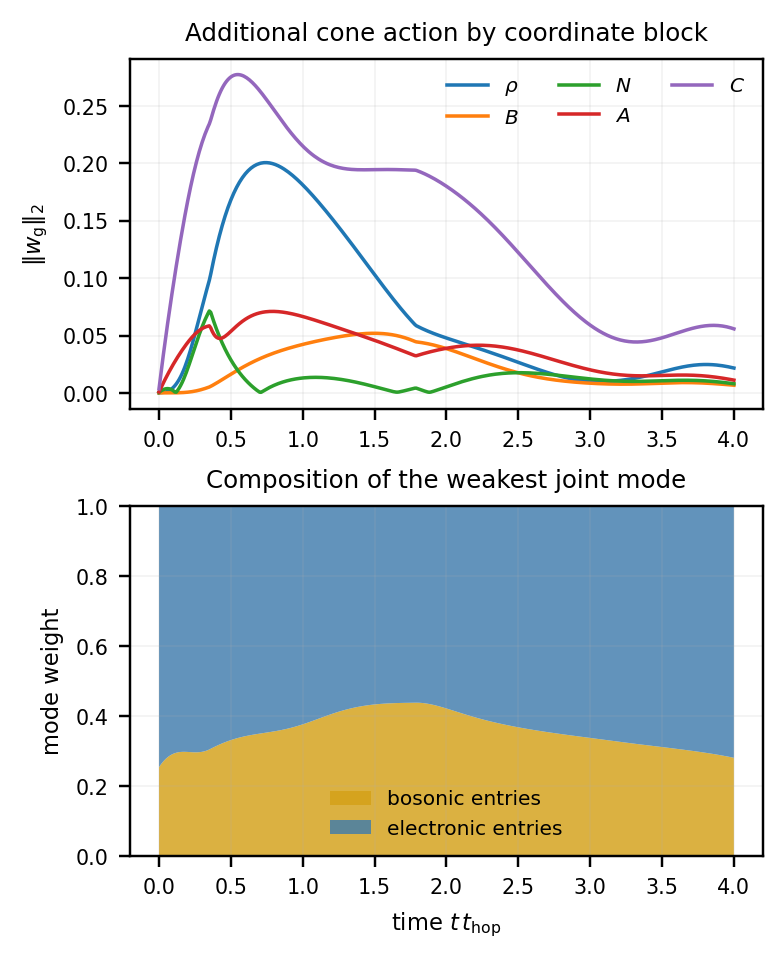
\includegraphics[width=0.82\linewidth]{MATH/paper_facing/paper_V_high_u_gkba/pedagogical/figures/joint_electron_phonon_mechanism_evidence.png}
        \caption{Correction mechanism. Upper: the part of \(w\) required by joint-Gram positive semidefiniteness beyond the trace and energy equalities, resolved by coordinate block (\(69.18\%\) \(C\), \(23.37\%\) \(\rho\)). Lower: the normalized eigenvector associated with \(\lambda_{\min}(\mathcal G)\), resolved as \(62.97\%\) electronic and \(37.03\%\) bosonic.}
        \label{fig:paper-v-mechanism}
    \end{minipage}
\end{figure}

\end{document}
